\chapter{STARPY: Bayesian inference of a galaxy's star formation history}\label{chap:starpy}

\emph{The work in the following chapter has been published in \citet{smethurst15}.}
\\

\section{Star Formation History Models}\label{qmod}

The quenched star formation history (SFH) of a galaxy can be simply modelled as an exponentially declining star formation rate (SFR) across cosmic time as:
\begin{equation}\label{sfh}
SFR =
\begin{cases}
I_{sfr}(t_q) & \text{if } t \leq t_q \\
I_{sfr}(t_q) \times exp{\left( \frac{-(t-t_{q})}{\tau}\right)} & \text{if } t > t_q 
\end{cases}
\end{equation}
where $t_{q}$ is the onset time of quenching, $\tau$ is the timescale over which the quenching occurs and $I_{sfr}$ is an initial constant star formation rate dependent on $t_q$.  A smaller $\tau$ value corresponds to a rapid quench, whereas a larger $\tau$ value corresponds to a slower quench. This model is clearly not a fully hydrodynamical simulation, it is a deliberately simple model built in order to test our understanding of the evolution of galaxy populations. This SFH model has previously been shown to appropriately characterise quenching galaxies \citep{weiner06, Martin07, noeske07,schawinski14}. However. it is not expected to accurately determine the SFH of every galaxy in the \textsc{gz2-galex} sample, in particular galaxies which have not undergone any quenching. 

Here, I assume that all galaxies formed at a time $t=0~\rm{Gyr}$ with an initial burst of star formation, $I_{sfr}(t_q)$. This initial constant star formation rate must be defined in order to ensure the `model' galaxy  has a reasonable stellar mass by $z\sim0$. This value will be dependent on the epoch at which quenching is modelled to occur, hence the dependence of this initial star formation rate on quenching time in Equation~\ref{sfh}. To tackle this problem, I looked to the literature; \citet[][Equation 1]{peng10} define a relation between the average specific SFR ($\rm{sSFR}=SFR/M_*$) and redshift by fitting to measurements of the mean sSFR of blue star forming galaxies from SDSS, zCOSMOS and literature values from \cite{Elbaz07} and \cite{daddi07} measured at increasing redshifts with data from the GOODS survey:
\begin{equation}\label{eq:peng}
sSFR(m,t) = 2.5 \left( \frac{m}{10^{10} M_{\odot}} \right)^{-0.1} \left(\frac{t}{3.5 ~\rm{Gyr}}\right)^{-2.2} \rm{Gyr}^{-1}.
\end{equation}
Beyond $z \sim 2$ the characteristic SFR flattens and is roughly constant back to $z\sim6$. This flattening can be seen across similar observational data \citep{peng10, gonzalez10, bethermin12}; the cause is poorly understood but may reflect a physical limit to the sSFR of a galaxy. 

Motivated by these observations, the relation defined in \citet{peng10} is taken up to a cosmic time of $t=3~\rm{Gyr}$ ($z \sim 2.3$) and prior to this the value of the sSFR at $t=3~\rm{Gyr}$ is used (see middle panel of Figure~\ref{sfr_mass_col}). At the point of quenching, $t_{q}$, the SFH models are therefore defined to have an $I_{sfr}(t_q)$ which lies on this relationship for the sSFR, for a galaxy with mass, $m = 10^{10.27} M_{\odot}$ (the mean mass of the \textsc{gz2-galex} sample; see left panel of Figure~\ref{sfr_mass_col}). This choice of $I_{sfr}(t_q)$ is an important one, however does not impact on the predicted colours output by the model (see below) as it is merely a normalisation factor on the SFH. $[t_q, \tau]$, which set the shape of the SFH, are the crucial parameters. 

\begin{figure*}
\centering{
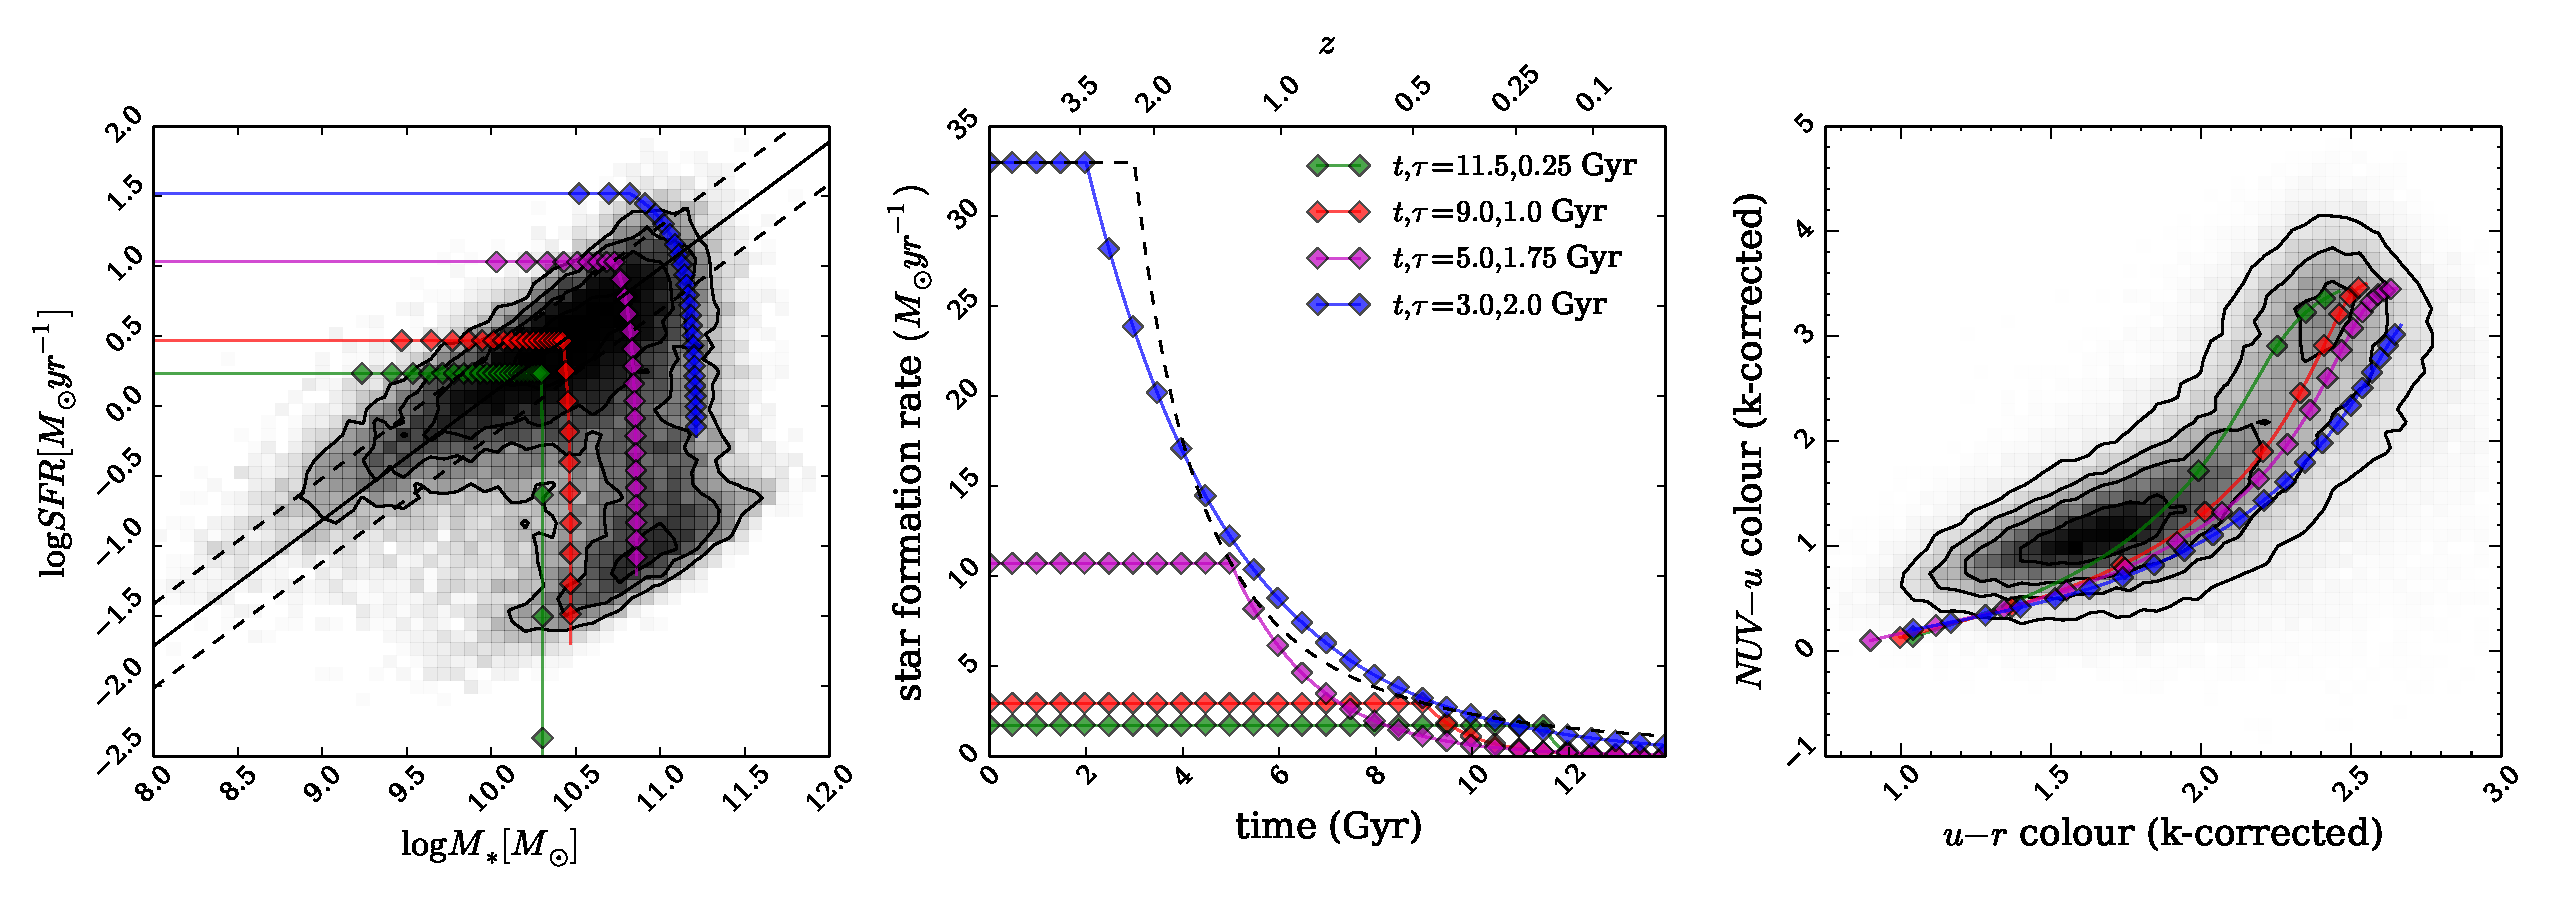
\includegraphics[width=\textwidth]{starpy/sfr_mass_colour_diagram.pdf}}
\caption[SFH models in observational planes]{Left panel: SFR-stellar mass plane for all 126,316 galaxies in the \textsc{gz2-galex} sample (shaded contours), with model galaxy trajectories shown by the coloured lines, with each point representing a time step of $0.5~\rm{Gyr}$.  The SFS as defined by \citet{peng10} is shown by the solid line with $\pm1\sigma$ (dashed lines). Middle panel: The SFHs of the models are shown, where the SFR is initially constant before quenching at time $t_q$ and thereafter exponentially declining with a characteristic timescale $\tau$. The SFR at the point of quenching is set to be consistent with the typical SFR of a star-forming galaxy at the quenching time, $t_q$ (dashed curve; \citealt{peng10}). Right panel: The full range of models can reproduce the observed colour-colour properties of the \textsc{gz2-galex} sample; for clarity the figures show only 4 of the possible models explored in this study. Note that some of the model tracks produce colours redder than the apparent peak of the red sequence in the GZ2 subsample; however this is not the true peak of the red sequence due to the necessity for NUV colours from GALEX (see Section \ref{defGV}.) {\minor The numbers indicate contour levels and the median error on each measured parameter is shown in the bottom right of each panel where relevant.}}
\label{sfr_mass_col}
\end{figure*}
  
Under these assumptions the average SFR of these models will result in a lower value than the relation defined in \citet{peng10} at all cosmic times as each galaxy only resides on the SFS at the point of quenching. However galaxies cannot remain on the SFS from early to late times throughout their entire lifetimes given the unphysical stellar masses and SFRs that would result in the local Universe \citep{bethermin12, Heinis14}. If prescriptions for starbursts, mergers, AGN etc. were included in this model, the reproduction of the average SFR across cosmic time would improve; however I have chosen to focus first on the simplest possible model.

Once this SFH is obtained, it is convolved with the \citet{BC03} population synthesis models to generate a model SED at each time step. The observed features of galaxy spectra can be modelled using simple stellar population techniques which sum the contributions of individual, coeval, equal-metallicity stars. The accuracy of these predictions depends on the completeness of the input stellar physics. Comprehensive knowledge is therefore required of (i) stellar evolutionary tracks and (ii) the initial mass function (IMF) to synthesise a stellar population accurately. 

These stellar population synthesis (SPS) models are an extremely well explored (and often debated) area of astrophysics \citep{Maraston05, Eminian08, CGW09, falkenberg09, chen10, kriek10, miner11, melbourne12}. In this work I have chosen to utilise the \citet{BC03} \emph{GALEXEV} SPS models, along with a Chabrier IMF \citep{chabrier03}, across a large wavelength range ($0.0091 < ~\lambda~\rm{[\mu m]}~ < 160 $) with solar metallically (m62 in the \citet{BC03} models; hereafter BC03), to allow a direct comparison with \citet{schawinski14}.


Flux from stars younger than $3~$Myr in the SPS model is suppressed to mimic the large optical depth of protostars embedded in dusty formation clouds (as in \citealt{schawinski14}).  Filter transmission curves are then applied to the fluxes to obtain AB magnitudes and ultimately colours.  For a particular galaxy at an observed redshift, $z$, I calculate the observed time, $t^{obs}$, for that galaxy using the standard cosmological conversion between redshift and time provided in the \textsc{astropy} {\em Python} module \citep{astropy13}. The predicted colours of the SFH models at the observed redshift of each individual galaxy can then be compared to the observed colours directly, as in the right panel of Figure \ref{sfr_mass_col}. Note that some of the SFHs shown produce colours redder than the apparent peak of the red sequence in the \textsc{gz2-galex} sample; however this is not the true peak of the red sequence due to the necessity for NUV colours from GALEX (see Section \ref{defGV}). Star forming galaxies in this regime are fitted by a constant SFR up until $t_q \simeq t^{obs}$, with a very low probability.

\begin{figure}
\centering{
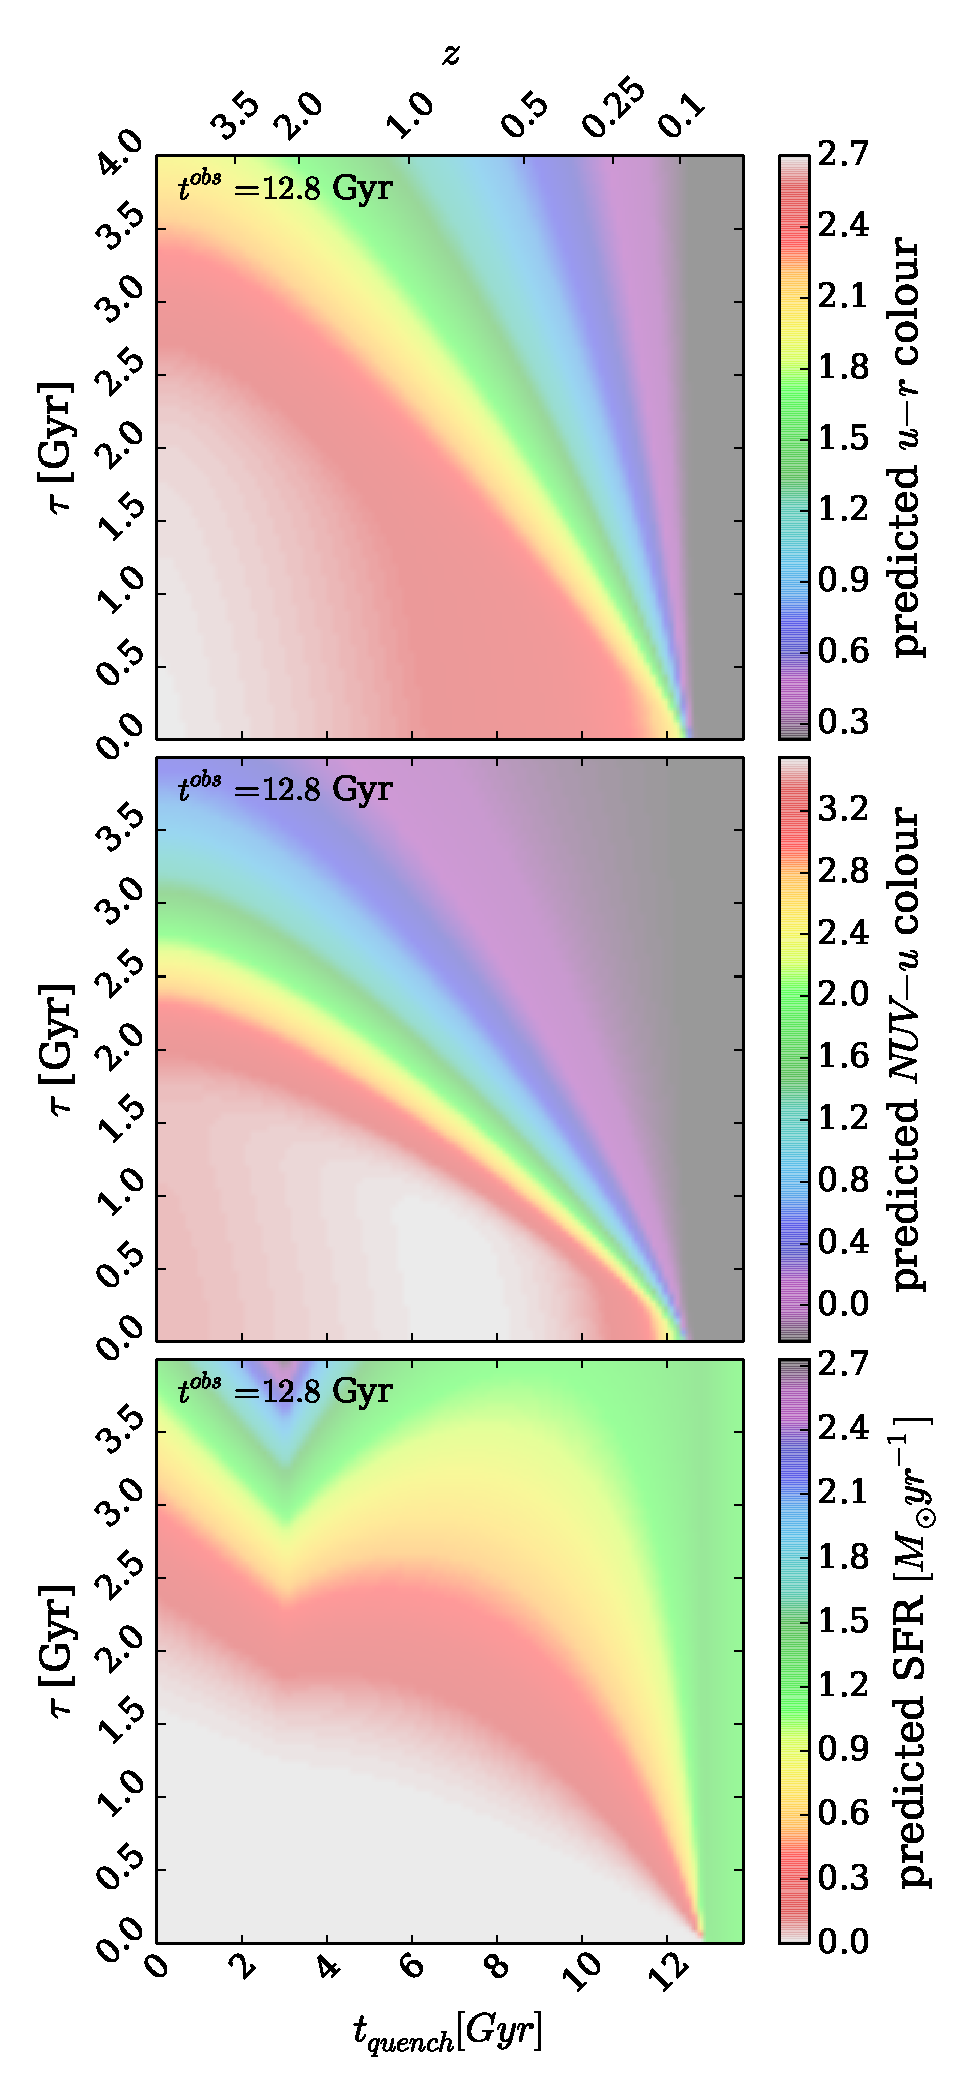
\includegraphics[height=0.75\textheight]{starpy/colours.pdf}}
\caption[Predicted colours and SFRs of quenching models]{Quenching timescale $\tau$ versus quenching onset time $t_q$ in all three panels for the quenched SFH models used in \starpy. Colour shadings show model predictions of the $u-r$ optical colour (top panel), $NUV-u$ colour (middle panel), and star formation rate (lower panel), at $t^{obs} = 12.8~\rm{Gyr}$, the mean observed redshift of the \textsc{gz2-galex} sample (see Section \ref{qmod}). The combination of optical and NUV colours is a sensitive measure of the $\theta = [t_q, \tau]$ parameter space. Note that all models with $t > 12.8$ \rm{Gyr} are effectively un-quenched. The `kink' in the bottom panel is due to the assumption that the sSFR is constant prior to $t \sim 3~\rm{Gyr}$ ($z\sim 2.2$).}
\label{pred}
\end{figure}

Figure~\ref{pred} shows these predicted optical and NUV colours at a time of $t^{obs} = 12.8 ~\rm{Gyr}$ (the mean observed time of the \textsc{gz2-galex} sample, $z \sim 0.076$) for the exponential SFH model. These predicted colours will be referred to as $d_{c,p}(t_{q}, \tau, t^{obs})$, where $c$=\{opt,NUV\} and $p$ = predicted. The SFR at a time of $t^{obs}=12.8~\rm{Gyr}$ is also shown in Figure~\ref{pred} to compare how this impacts on the predicted colours. The $u-r$ predicted colour shows an immediate correlation with the SFR, however the $NUV-u$ colour is more sensitive to the value of $\tau$ and so is ideal for tracing any recent star formation in a population. At small $\tau$ (rapid quenching timescales) the $NUV-u$ colour is insensitive to $t_{q}$, whereas at large $\tau$ (slow quenching timescales) the colour is very sensitive to $t_{q}$. Together the two colours are ideal for tracing the effects of $t_{q}$ and $\tau$ in a population. 


\section{Probabilistic Fitting Methods}\label{stats}

In order to achieve robust conclusions I conducted a Bayesian analysis \citep{Sivia, mackay03} of the predicted colours from the SFH models in comparison to the observed colours of the \textsc{gz2-galex} sample. 

\subsection{A short introduction to Bayesian statistics}

Frequentist statistics allows {\minor for the calculation of} the probability of an event (i.e. a hypothesis) occurring over many trials of an experiment. The accuracy of the derived probability is also dependant on the number of experiment trials conducted. Conversely, a Bayesian approach allows {\minor for the evaluation of} whether a hypothesis, $\theta$, is true, given the {\minor acquired} data, $d$, by relating this to something easily {\minor calculable}: the probability that {\minor the data would be observed} if the hypothesis was true. It does so by employing the rules of conditional probability into Bayes' theorem:
\begin{equation}\label{bayes}
P(\theta|d) \propto P(d | \theta)P(\theta),
\end{equation}
which is made up of three separate terms: 
\begin{enumerate}[(i)]
\item $P(\theta)$, known as the \emph{prior} probability which represents {\minor the} knowledge (or ignorance) about the hypothesis before {\minor the analysis of} any data. 
\item $P(d  | \theta)$, the \emph{likelihood} function which gives the probability of observing the data given the hypothesis being tested. 
\item $P(\theta | d)$, the \emph{posterior} probability which summarises {\minor the} knowledge of the hypothesis given {\minor the} observed data.
\end{enumerate}
The missing normalisation factor in Equation~\ref{bayes} doesn't explicitly depend on {\minor the} hypothesis and so doesn't have to be calculated for model parameter estimation problems (for example, where {\minor the} hypothesis, $\theta$, is a model described by some number of parameters with the goal of emulating {\minor the} data). Deciding on a prior and likelihood function is very much dependent on the problem {\minor to be solved}; the decision is often informed by {\minor the} knowledge of the problem. 

This difference between frequentist and Bayesian statistics is often highlighted by the example of a coin being tossed; if {\minor a coin is tossed} 10 times and {\minor produces} 3 heads ($H=3$) and 7 tails ($T=7$) what is the probability that the coin is weighted? {\minor Frequentist statistics is limited} by the fact that {\minor the coin was only tossed 10 times}; the experiment {\minor wasn't repeated} enough to be sure of {\minor the} response that the probability of tossing a tails,  $P(T)=0.7$. Perhaps if the coin {\minor had been tossed} $1000$ times and recorded $720$ tails then the {\minor statement that the coin is weighted is more certain}. Herein lies the problem of frequentist statistics; not only is {\minor the} answer dependent on the number of experiment trials but how likely {\minor an} answer is of being correct {\minor cannot be quantified}. 

\begin{figure}
\centering{
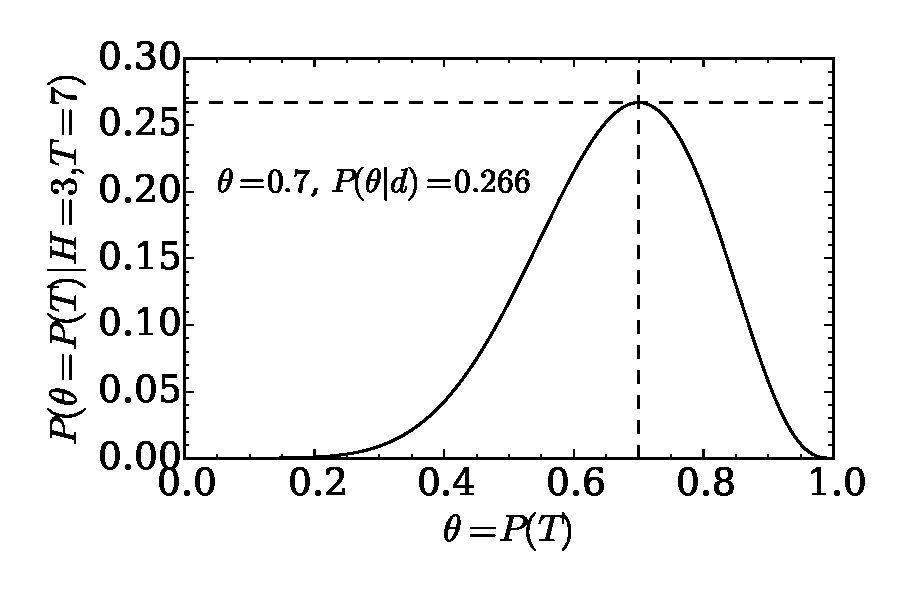
\includegraphics[width=0.49\textwidth]{starpy/prob_values_bias_coin.pdf}
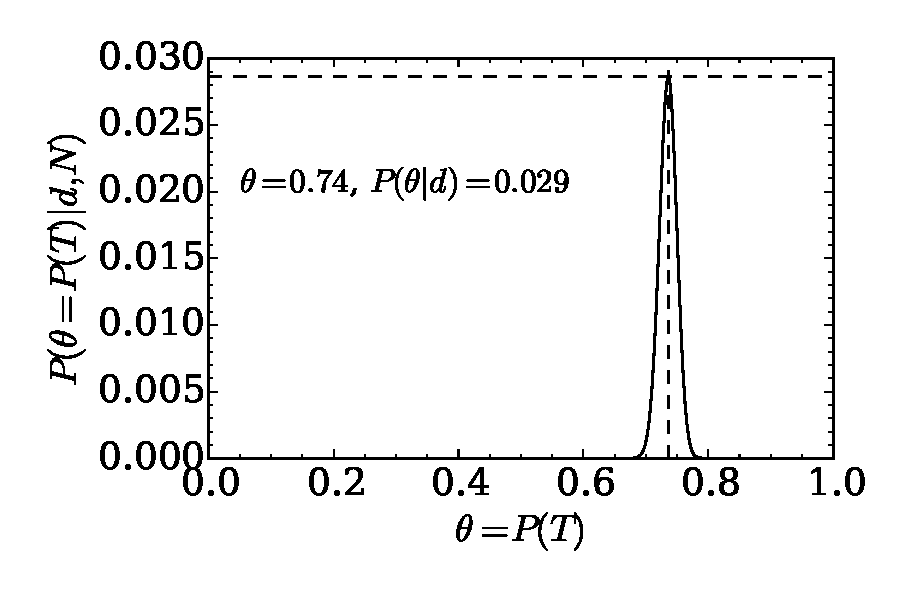
\includegraphics[width=0.49\textwidth]{starpy/prob_values_bias_coin_1000.pdf}}
\caption[Is my coin biased? An example of the strength of Bayesian statistics]{The unnormalised posterior probability calculated for multiple hypotheses for the probability of tossing a tails, $P(T)$ in the case of 10 data points (left) and 1000 data points (right). The dashed lines in both cases show the posterior probability values at the peak of the distribution.}
\label{fig:coin}
\end{figure}

Bayesian statistics {\minor allows this to be quantified}; first a likelihood, $P(d | \theta)$, and prior distribution, $P(\theta)$, {\minor must be chosen, however} there are many choices available. For example, given that most coins are not weighted, {\minor a sensible choice for a prior distribution would} be a Gaussian, centered on $P(T)=0.5$. Or, where all scenarios are equally likely, a flat prior distribution {\minor may be chosen}. 

The likelihood function {\minor is informed by} which hypothesis (or model, $\theta$) best describes the problem. In the {\minor case of the coin toss} a Bernouilli likelihood distribution may be chosen, e.g. 
\begin{equation}\label{bernouilli}
P(d  | \theta, N) = \theta^d~ (1-\theta)^{N-d}, 
\end{equation}
where $d$ is the number of tails flipped, $\theta$ is {\minor the} guess (or hypothesis) for $P(T)$, i.e. how biased the coin is, and $N$ is the number of flips of the coin. If this likelihood, $P(d | \theta, N)$ {\minor is calculated} for many possible values of $\theta = P(T)$ and multiplied {\minor by the} flat prior distribution, the {\minor result is the} unnormalised posterior probability distribution, shown in the left panel of Figure~\ref{fig:coin}. {\minor This distribution shows how} $P(T) = 0.7$ is indeed the most likely value for the probability of tossing a tails given the 10 data points {\minor acquired}. Not only has the best model to describe the coin {\minor been determined} given the {\minor aquired} data, but also {\minor a description of} how certain this model is (since this is an unnormalised posterior distribution a definitive probability {\minor can't be given but can be quoted} in comparison to other $\theta$ values). As the number of trials in the experiment, $N$, {\minor is increased the result becomes more certain}, as in the right panel of Figure~\ref{fig:coin}. 

This is the strength of using a Bayesian method over a frequentist one. In particular, the output of a Bayesian analysis is probabilistic in nature, returning the posterior probability distribution across the model parameter space, $\theta$ (in the example in Figure~\ref{fig:coin} this is demonstrated in one dimension, but this can be visualised over as many dimensions as needed in the problem). This distribution encodes a huge amount of useful information that can be utilised in the analysis of the hypothesis. 

Since this investigation is focussed on finding the most likely star formation history model in a very degenerative parameter space for a large sample of galaxies, the obvious choice of method for analysis is therefore a Bayesian one.  


\subsection{STARPY}

For the SFH problem at hand, using this Bayesian approach requires consideration of all possible combinations of the model parameters $\theta \equiv (t_{q}, \tau)$ (the hypothesis in this instance). Assuming that all galaxies formed at $t=0~\rm{Gyr}$, we can assume that the `age' of each galaxy in the GZ2 sample is equivalent to an observed time, $t^{obs}_{k}$. I then used this  `age' to calculate the predicted model colours at this cosmic time for a given combination of $\theta$: $d_{c,p}(\theta_k, t^{obs}_{k})$ for both optical and NUV $(c={opt,NUV})$ colours. The predicted model colours can now directly be compared with the observed \textsc{gz2-galex} sample colours, so that for a single galaxy $k$ with optical ($u-r$) colour, $d_{opt, k}$ and NUV ($NUV-u$) colour, $d_{NUV,k}$,  I have chosen the likelihood of a given model $P(d_{k}|\theta_k, t^{obs}_{k})$ to be:


\begin{equation}\label{like}
\begin{split}
P(d_{k}|\theta_k, t^{obs}_{k}) = \frac{1}{\sqrt{2\pi\sigma_{opt, k}^2}}\frac{1}{\sqrt{2\pi\sigma_{NUV, k}^2}} \exp{\left[ - \frac{(d_{opt, k} - d_{opt, p}(\theta_k, t_{k}^{obs}))^2}{\sigma_{opt, k}^2} \right]} \\ \exp{\left[ - \frac{(d_{NUV, k} - d_{NUV, p}(\theta_k, t_{k}^{obs}))^2}{\sigma_{NUV, k}^2} \right]}.
\end{split}
\end{equation}


Here I have assumed that $P(d_{opt}|\theta_k, t^{obs}_{k})$ and $P(d_{NUV}|\theta_k, t^{obs}_{k})$ are independent of each other and that the errors on the observed colours are also independent. To obtain the probability of a combination of $\theta$ values given the data: $P(\theta_k|d_k, t^{obs})$, i.e. how likely a single SFH model is  given the observed colours of a single \textsc{gz2-galex} galaxy, I utilise Bayes' theorem as:
 \begin{equation}\label{big}
P(\theta_k|d_k, t^{obs}) = \frac{P(d_k|\theta_k, t^{obs})P(\theta_k)}{\int P(d_k |\theta_k, t^{obs})P(\theta_k) d\theta_k}.
\end{equation}
I assume a flat prior on the model parameters so that:
\begin{equation}\label{prior}
P(\theta_k) =
\begin{cases}
1 & \text{if } 0 \leq t_q ~\rm{[Gyr]}~ \leq 13.8 ~  \text{ and } ~ 0 \leq \tau  ~\rm{[Gyr]}~ \leq 4\\
0 & \text{otherwise.} \\
\end{cases}
\end{equation}

\begin{figure}
\centering{
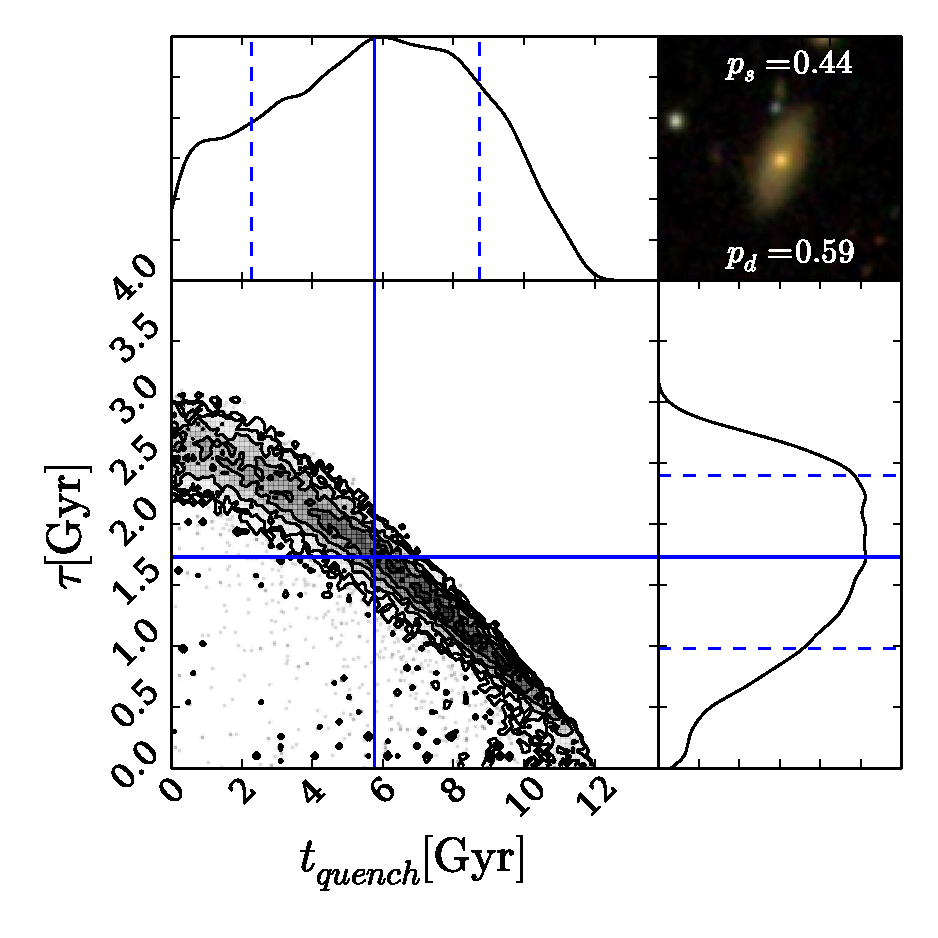
\includegraphics[width=0.9\textwidth]
{starpy/triangle_t_tau_red_s_1237655504035185152_40000_14_16_06_08_14.pdf}}
\caption[Example \starpy ~output]{Example output from \starpy ~for a galaxy within the red sequence. The contours show the positions of the `walkers' in the Markov Chain (which are analogous to the areas of high probability) for the quenching models described by $\theta = [t_q, \tau]$. The histograms show the 1D projection along each axis. Solid (dashed) blue lines show the best fit parameters (with $\pm 1\sigma$) to the data. The postage stamp image from SDSS is shown in the top right along with the debiased vote fractions for smooth ($p_s$) and disc ($p_d$) from Galaxy Zoo 2. {\minor The contours bound $12\%$, $40\%$, $68\%$ and $86\%$ of the walker positions}.}
\label{one_example}
\end{figure}

As the denominator of Equation~\ref{big} is a normalisation factor, comparison between likelihoods for two different SFH models (i.e., two different combinations of $\theta_k = [t_q, \tau]$) is equivalent to a comparison of the numerators. Markov Chain Monte Carlo (MCMC; \citealt{mackay03, emcee13, GW10}) analysis provides a robust comparison of the likelihoods between $\theta$ values.

MCMC allows for a more efficient exploration of the parameter space by avoiding those areas with low likelihood. A large number of `walkers' are started at an initial position (i.e. an initial hypothesis, $\theta$), where the likelihood is calculated; from there they individually `jump' a randomised distance to a randomised new area of parameter space. If the likelihood in this new position is greater than the original position then the `walkers' accept this change in position. Any new position then influences the direction of the  `jumps' of other walkers (this is the case in ensemble MCMC as used in this investigation but not for simple MCMC, which is much slower at converging). This is repeated for the defined number of steps after an initial `burn-in' phase. The length of this burn-in phase is determined after sufficient experimentation to ensure that the `walkers' have converged on a region of parameter space. I chose to use \emph{emcee},\footnote{\url{dan.iel.fm/emcee/}} a Python module which implements an affine invariant ensemble sampler to explore the parameter space, written by \cite{emcee13}. \emph{emcee} outputs the positions of these `walkers' in the parameter space, which are analogous to the regions of high posterior probability. 

I used the \emph{Python} programming language to code the routine outlined above into a package named \starpy ~which has been released with an open source license\footnote{\url{github.com/zooniverse/starpy}}. {\minor The required inputs for \starpy~ to run on a single galaxy	 are as follows: the $u-r$ colour, the error on $u-r$, the $NUV-u$ colour, the error on $NUV-u$ and the redshift, $z$. The output from \starpy~ is the two dimensional MCMC chain charting the $[t_q, \tau]$ positions of the walkers around parameter space. From this, `best fit' $[t_q, \tau]$ values along with their uncertainties can be determined from the median and $\pm1\sigma$ values of the walker positions.} An example output from \starpy~for a single galaxy from the \textsc{gz2-galex} sample in the red sequence is shown in Figure~\ref{one_example} wherein the degeneracies of the SFH model can be clearly seen and reflect those seen in the colours in Figure \ref{pred}. These degeneracies are present for all galaxies run through \starpy\ therefore if differences in the distributions arise when comparing two galaxies (or two populations), this is due to intrinsic differences in their SFHs and not due to the degeneracies of the model. 

\section{Testing STARPY}

\begin{figure}
\centering{
\includegraphics[width=\textwidth]{starpy/mosaic_test.jpg}}
\caption[Testing \starpy]{Results from \starpy ~for an array of synthesised galaxies with known, i.e. true, $t_q$ and $\tau$ values (marked by the red lines) using the complete function to calculate the predicted colour of a proposed set of $\theta$ values in each MCMC iteration, assuming an error on the calculated known colours of $\sigma_{u-r} = 0.124$ and $\sigma_{NUV-u} = 0.215$ (the average errors on the \textsc{gz2-galex} sample colours). I also assume that each synthesised galaxy has been observed at a redshift of $z=0$. In each case \starpy ~succeeds (50th percentile best fit parameters are shown by the blue lines) in locating the true parameter values within the degeneracies of the star formation history model. {\minor The contours bound $12\%$, $40\%$, $68\%$ and $86\%$ of the walker positions in each panel}.}
\label{test_mosaic}
\end{figure}

In order to test that \starpy ~can find the correct quenching model for a given observed colour, 25 synthesised galaxies were created with known SFHs (i.e. known values of $\theta = [t_q, \tau]$) from which optical and NUV colours were generated using the BC03 SPS models. These were input into \starpy ~ to test whether the known values of $\theta$ were reproduced, within error, for each of the 25 synthesised galaxies. Figure~\ref{test_mosaic} shows the results for each of these synthesised galaxies, with the known values of $\theta$ shown by the red lines (the largest difference between the known and derived values being $[\Delta t_q, \Delta \tau] \approxeq [4.5, 2.0]$). In some cases this red line does not coincide with the inferred best fit $\theta$ values shown by the blue lines, however in all cases the intersection of the red lines (i.e. the known or true values input) resides within the parameter space explored by the walkers, which trace the region of highest posterior probability. Therefore \starpy\ succeeds in locating the true parameter values within the degeneracies of the SFH model. 

\section{Speeding up STARPY}\label{lookuptable}

\begin{figure*}
\centering{
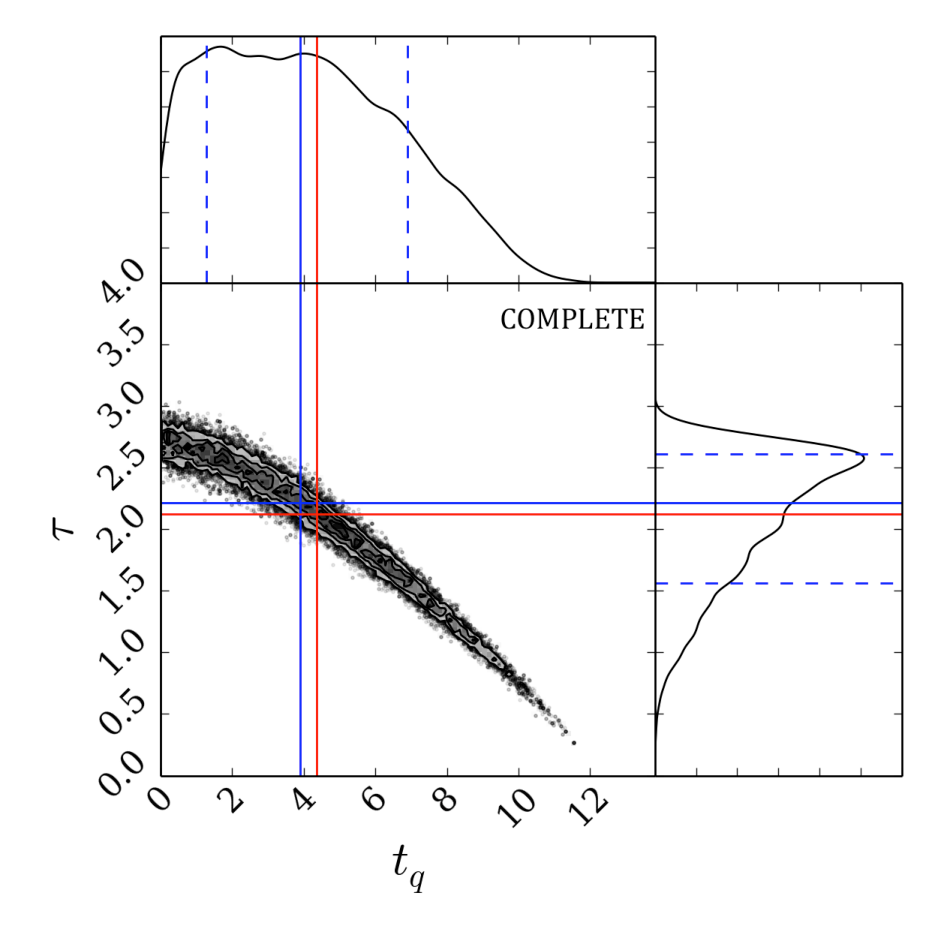
\includegraphics[width=0.49\textwidth]{starpy/corner_test_starfpy_full_sfh_function_0.pdf}
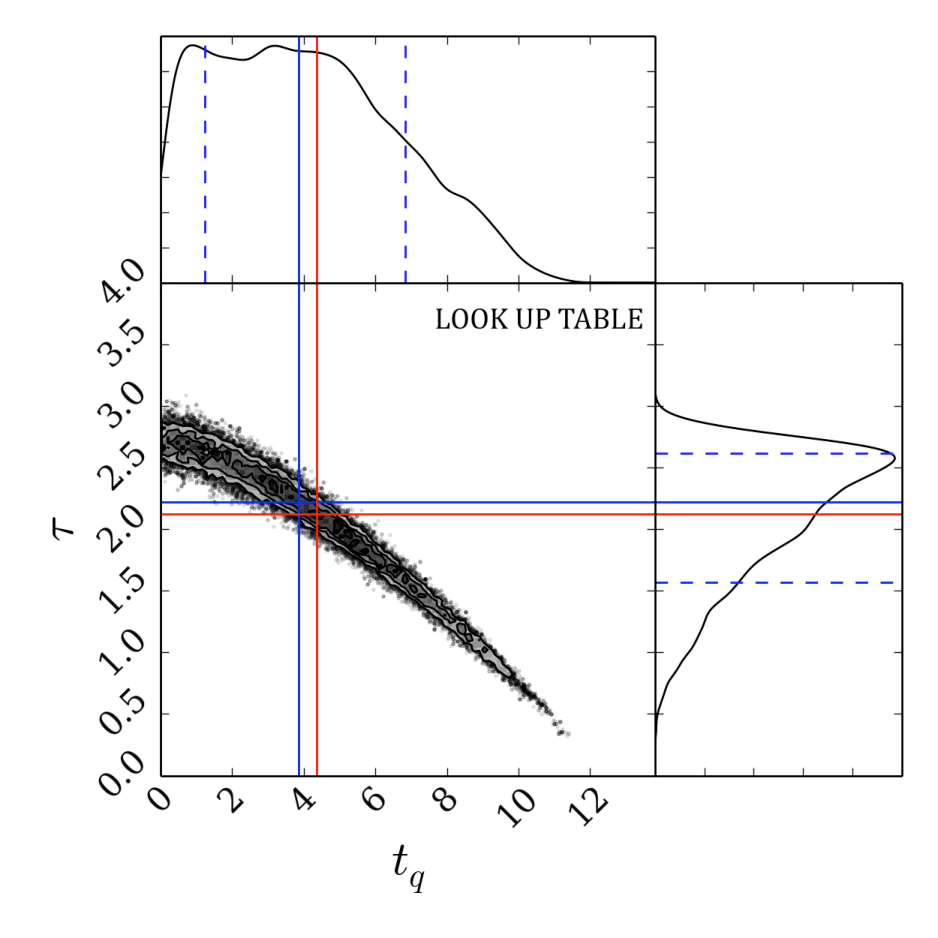
\includegraphics[width=0.49\textwidth]{starpy/corner_test_starfpy_lookup_0.pdf}}
\caption[Comparing complete and look-up table versions of \starpy]{Left panel: Results from \starpy ~for true $t_q$ and $\tau$ values (red lines) using the complete function to calculate the predicted colour of a proposed set of $\theta$ values in each MCMC iteration. The median walker position (the 50th percentile of the Bayesian probability distribution) is shown by the solid blue line with the dashed lines encompassing $68\%~(\pm 1\sigma)$ of the samples (the 16th and 84th percentile positions). The time taken to run for a single galaxy using this method is approximately 2 hours. Right panel: Results from \starpy ~for true $t_q$ and $\tau$ values using a look up table generated from the complete function to calculate the predicted colour of a proposed set of $\theta$ values in each MCMC iteration. The time taken to run for a single galaxy using this method is approximately 2 minutes. {\minor The contours bound $12\%$, $40\%$, $68\%$ and $86\%$ of the walker positions in each panel}.}
\label{lookup}
\end{figure*}

\begin{table}
\centering{
\caption{Median walker positions (the 50th percentile; as shown by the blue solid lines in Figure~\ref{lookup}) found by \starpy\ for a single galaxy, using the complete star formation history function and a look up table to speed up the run time. The errors quoted define the region in which $68\%$ of the samples are located, shown by the blue lines in Figure~\ref{lookup}. The known true values are also quoted, as shown by the red lines in Figure~\ref{lookup}. All values are quoted to three significant figures.}
\label{table:median_lu}
\begin{tabular*}{0.65\textwidth}{r @{\extracolsep{\fill}}ccc}
\multicolumn{1}{l}{} & \multicolumn{3}{c}{}                                          \\ \hline
                     & $t_q$                       & $\tau$                       &  \\ \hline
True                 & $4.37$                        & $2.12$                         &  \\
Complete             & $3.89 \pm^{3.01}_{2.62}$ & $2.21 \pm^{0.39}_{0.65}$ &  \\
Look up table        & $3.85 \pm^{2.98}_{2.61}$ & $2.21 \pm^{0.39}_{0.64}$ & \\ \hline
\end{tabular*}}
\end{table}

I wish to consider the SFH model parameters for a large populations of galaxies across the colour magnitude diagram. However for each combination of $\theta$ values which \emph{emcee} proposes for a single galaxy, a new SFH must be built, prior to convolving it with the BC03 SPS models at the observed age and then predicted colours calculated from the resultant SED. For a single galaxy this takes up to 2 hours on a typical desktop machine for long Markov Chains. A 3-dimensional look-up table was therefore generated at $50 ~t^{obs}$, $100 ~t_{quench}$ and $100 ~\tau$ values which were interpolated over for a given observed galaxy's age and proposed $\theta$ values at each step in the Markov Chain. This ensured that a single galaxy SFH takes approximately 2 minutes to infer on a typical desktop machine. 

Figure~\ref{lookup} shows one example of how using the look up table in place of the full function does not affect the results to a significant level. Table~\ref{table:median_lu} quotes the median walker positions (the 50th percentile of the Bayesian probability distribution) along with their $\pm 1\sigma$ ranges for both methods in comparison to the true values specified to test \starpy. The uncertainties incorporated into the quoted values by using the look up table are therefore minimal with a maximum $\Delta = 0.043$ (the difference between the complete \& look up table derived values quoted in Table~\ref{table:median_lu}). This test was run with $1000$ randomised $[t_q, \tau]$ values across the entire parameter space; the example shown in Figure \ref{lookup} (with values quoted in Table~\ref{table:median_lu}) was found to have the largest difference, $\Delta$, between complete and look up table derived values. 

Using this lookup table, each of the $126,316$ total galaxies in the \textsc{gz2-galex} sample was run through \starpy ~on multiple cores of a computer cluster to obtain the Markov Chain positions (analogous to $P(\theta_k|d_k)$) for each galaxy, $k$ (see Figure~\ref{one_example}). In each case the Markov Chain consisted of $100$ `walkers' which took $400$ steps in the `burn-in' phase and $400$ steps thereafter, at which point the MCMC acceptance fraction was checked to be within the range $0.25 < f_{acc} < 0.5$ (the fraction of proposed walker `jumps' that were accepted), which was true in all cases. This acceptance fraction ensures that the walkers are sampling the probability space correctly as they explore. If $f_{acc} \sim 0$ then all the walker jumps are rejected and so the walkers won't move from their initial starting positions and the output will not represent the posterior distribution accurately. If $f_{acc} \sim 1$ then all jumps are accepted and the walkers will just perform a random walk around the parameter space, which again will not represent the posterior distribution accurately. The range of $0.25 < f_{acc} < 0.5$ used in this case is the general rule of thumb stated by \citet*{gelman96}.


\section{POPSTARPY: studying populations of galaxies with STARPY}\label{popstarpy}

To study the SFH of a large population of galaxies, the individual galaxy walker positions output by \starpy ~(analogous to the posterior probability distribution) are combined across $[t_q, \tau]$ space. The Markov Chain walker positions are binned and weighted by their corresponding logarithmic posterior probability $\log [P(\theta_k|d_k)]$, provided by the \emph{emcee} package, in order to emphasise the features and differences between various populations. This weighting by $\log [P(\theta_k|d_k)]$ is to minimise the contribution of galaxies poorly fit by this exponentially declining SFH (e.g. star forming galaxies). This is no longer inference of model parameters but merely a method to visualise the results across a population of galaxies (see Section~\ref{althyper}).

I also discard those walker positions with a corresponding normalised posterior probability of $P(\theta_k|d_k) < 0.2$ in order to exclude galaxies which are not well fit by the quenching model. Therefore, galaxies which reside on the SFS will not contribute to the final population distribution of quenching parameters. This raises the issue of whether I exclude a significant fraction of the \textsc{gz2-galex} sample and whether those galaxies reside in a specific location of the colour-magnitude diagram. The number of galaxies in a population which had all or more than half of their walker positions discarded due to low probability are shown in Table \ref{discardnum}. Using the $P(\theta_k|d_k) < 0.2$ constraint, $2.4\%$, $7.0\%$ and $5.4\%$ of green, red and blue galaxies respectively had all of their walker positions discarded. 

This is not a significant fraction of any population, hence the \starpy~module is effective in fitting the majority of galaxies and this method of discarding walker positions ensures that poorly fit galaxies are removed from the analysis of the results. Figure \ref{discarded} shows that these galaxies with discarded walker positions are also scattered across the optical-NUV colour-colour diagram and therefore \starpy~is also effective in fitting galaxies across this entire plane. The galaxies that are discarded can be seen to mostly lie outside the contours of the \textsc{gz2-galex} sample in the colour-colour plane shown in Figure~\ref{discarded}. This is due to the SPS models used to produce the SEDs of the model SFHs; these models are calibrated with typical galaxies rather than the extremes of galaxy evolution. Those galaxies with blue optical colours but red NUV colours, or vice versa, are oddities which cannot be explained by the SPS models and so \starpy~has particular difficulty fitting a SFH to these galaxies. 

{\minor There is also a possibility that a particular class of galaxies may be systematically discarded, for example, the rare \citep[$<1\%$;][]{Wong12, wild16} post-starburst phase. Such a system is often referred to as an `E+A' galaxy, as their spectra are a combination of a typical {\minor early-type} galaxy with added A star signatures due to their post starburst nature. These galaxies are therefore likely to have blue optical but red NUV colours, placing them in the typically discarded area of the colour magnitude diagram (see left hand panels of Figure~\ref{discarded}). This is apparent since a starburst with a subsequent quench will not be well fit by a SFH with a constant SFR followed by an exponential decline.}

\begin{table*}
\centering{
\caption{The number of galaxies in each population which had walker positions discarded due to low posterior probability values in order to exclude those galaxies from the analysis which were poorly fit by the SFH quenching model.}
\label{discardnum}
\begin{tabular*}{0.95\textwidth}{p{4cm} @{\extracolsep{\fill}} ccc}
                                          & \textbf{Red Sequence}                                   & \textbf{Green Valley}                                  & \textbf{Blue Cloud}                                      \\ \hline
All walkers discarded                     & \begin{tabular}[c]{@{}c@{}}1420\\ (7.00\%)\end{tabular} & \begin{tabular}[c]{@{}c@{}}437\\ (2.41\%)\end{tabular} & \begin{tabular}[c]{@{}c@{}}3109\\ (5.37\%)\end{tabular}  \\
More than half walker positions discarded & \begin{tabular}[c]{@{}c@{}}2010\\ (9.92\%)\end{tabular} & \begin{tabular}[c]{@{}c@{}}779\\ (4.30\%)\end{tabular} & \begin{tabular}[c]{@{}c@{}}6669\\ (11.52\%)\end{tabular} \\ \hline
\end{tabular*}}
\end{table*}

\begin{figure}
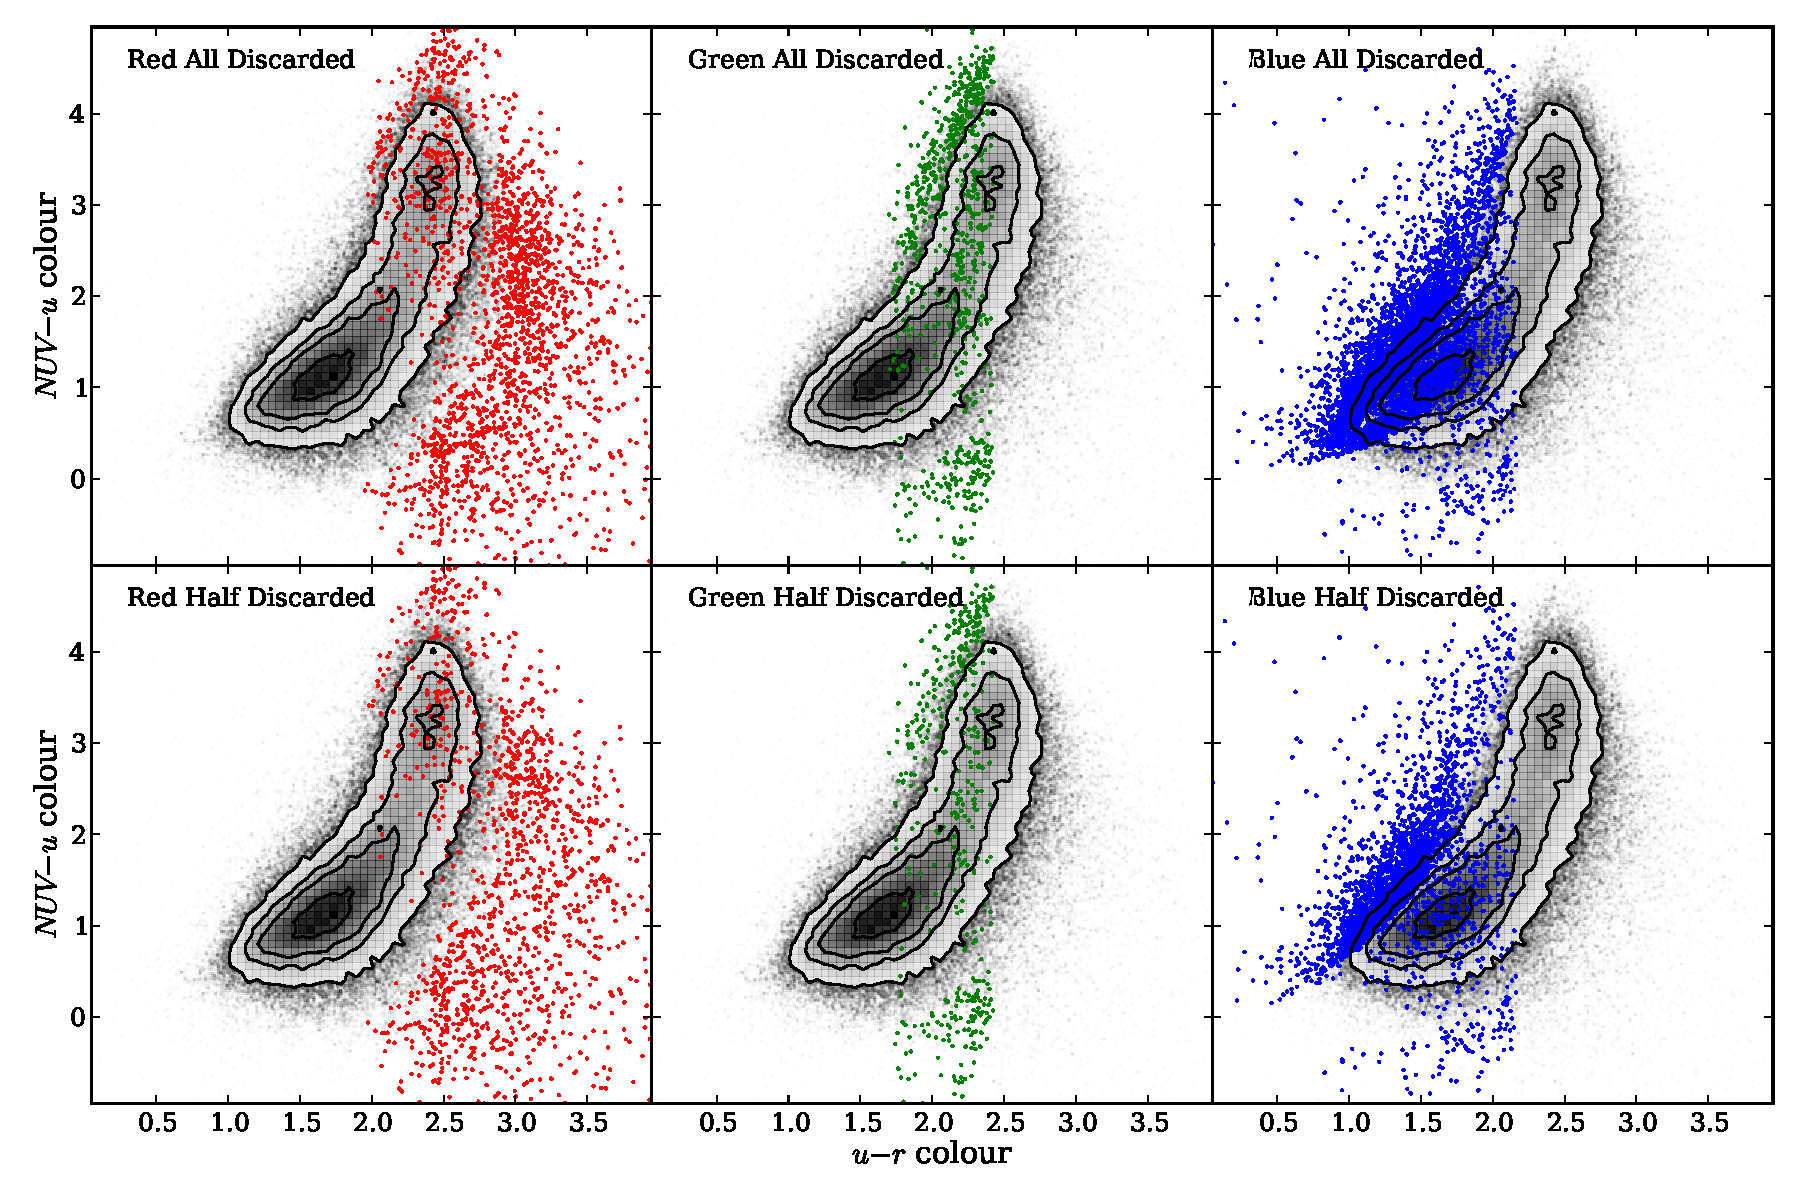
\includegraphics[width=0.9\textwidth]{starpy/discarded_galaxy_colour_colour.pdf}
\caption[Colours of discarded galaxies]{Contours show the \textsc{gz2-galex} sample optical-NUV colour-colour diagram. The points show the positions of the galaxies which had all (top panels) or more than half (bottom panel) of their walker positions discarded due to their low probability for the red sequence (left), green valley (middle) and blue cloud (right). {\minor Galaxies are typically discarded if they lie outside of the representative galaxy colour contours, for example, those galaxies with blue optical but red NUV colours, such as post starburst (or `E+A') galaxies.}}
\label{discarded}
\end{figure}

Figure~\ref{test_mosaic} shows how peaks in the histograms are found across all areas of the parameter space in both dimensions $[t_q, \tau]$, ensuring that any conclusions drawn from combined population distributions are due to a superposition of extended probability distributions, as opposed to a bimodal distribution of probability distributions across all galaxies.

I also utilise the GZ2 debiased user vote fractions to obtain separate population density distributions for both smooth and disc galaxies. This is obtained by also weighting by the morphology vote fraction of each individual galaxy when the binned walker positions of each galaxy in a population are combined. This ensures that the entirety of the \textsc{gz2-galex} sample is used, negating the need for a threshold on the GZ2 vote fractions \citep[e.g., $p_d > 0.8$ as used in][]{schawinski14} to give two definitively separate disc and smooth galaxy populations. This ensures that those galaxies of intermediate morphology are still included in the analysis. The walkers of those galaxies with a higher morphological vote fraction, $p_d$, are weighted more heavily and so contribute more to the disc weighted combined walker distributions (and similarly with $p_s$ for the smooth weighted combined walker distributions). These distributions will be referred to as the population densities.

For example, the galaxy shown in Figure~\ref{one_example} would contribute almost evenly to both the smooth and disc parameters due to the GZ2 vote fractions. Since galaxies with similar vote fractions contain both a bulge and disc component, this method is effective in incorporating intermediate galaxies which are thought to be crucial to the morphological changes between early- and late-type galaxies. It was the consideration of these intermediate galaxies which was excluded from the investigation by \citet{schawinski14}.

\subsection{Alternative Hierarchical Bayesian approach}\label{althyper}

The approach presented above relies upon a visualisation of the SFHs across each population, with no inference involved beyond the use of \starpy\ to derive the individual galaxy SFHs. An alternative approach to this problem would be to use a hierarchical Bayesian method to determine the `hyper-parameters' that describe the distribution of the parent population $\theta' = [t_q', \tau']$ that each individual galaxy's SFH is drawn from. 

The posterior PDF for $\vec{\theta}'$ to describe such a galaxy population:
\begin{equation}\label{hyper}
P(\vec{\theta}'|\vec{d}) = \frac{P(\vec{d}|\vec{\theta}')P(\vec{\theta}')}{P(\vec{d})}, 
\end{equation}
where $\vec{d}$ represents all of the optical and NUV colour data in a population $\{\vec{d}_k\}$. For one galaxy, $k$, the marginalised likelihood is:
\begin{equation}\label{one}
P(d_k|\vec{\theta}') = \iint \! P(d_k|t_k, \tau_k) P(t_k, \tau_k|\vec{\theta}') \ \mathrm{d}t_k ~ \mathrm{d}\tau_k
\end{equation}
and for all galaxies, $N$, therefore: 
\begin{equation}
P(\vec{d}|\vec{\theta}') = \prod_k^N P(d_k|\vec{\theta}').
\end{equation}

Using \starpy\ for an individual galaxy, $k$ the output is the `interim' posterior $P(t_k, \tau_k|d_k)$ which I can relate to $P(d_k|t_k, \tau_k)$  so that:

\begin{equation}\label{marg}
P(d_k|\vec{\theta}') = \iint  \! P(t_k, \tau_k|d_k) . P(d_k) . \frac{P(t_k, \tau_k|\vec{\theta}')}{P(t_k, \tau_k)} \ \mathrm{d}t_k ~ \mathrm{d}\tau_k.
\end{equation}
In order to calculate this I draw $N_s$ random samples, $r$, from each interim posterior, $P(t_k, \tau_k|d_k)$ so that Equation \ref{marg} can be expressed as a sum over a number of random samples, $N_s$ (as with the calculation of an expected mean):
\begin{equation}\label{imp}
P(d_k|\vec{\theta}') = \frac{P(d_k)}{N_s} \sum_r^{N_s} \frac{P(t_{k,r}, \tau_{k,r}|\vec{\theta}')}{P(t_k, \tau_k)},
\end{equation}
for the $r^{th}$ sample of $N_s$ total samples taken from one galaxy's, $k$,  interim posterior PDF. This fraction is known as the `importance weight', $w_r$, in importance sampling. 

However, I also have two morphological vote fractions that I can weight by to determine separate hyper-parameters, $\vec{\theta}' = [\vec{\theta}'_d, \vec{\theta}'_s]$, for both disc, $d$, and smooth, $s$, galaxies. Therefore:

\begin{equation}\label{morphimp}
w_r = \frac{P(t_{k,r}, \tau_{k,r}|\vec{\theta}')}{P(t_k, \tau_k)} =  \frac{p_{d,k} P(t_{k,r}, \tau_{k,r}|\vec{\theta}'_d) + p_{s,k} P(t_{k,r}, \tau_{k,r}|\vec{\theta}'_s)}{P(t_k, \tau_k)}
\end{equation} 

If we substitute equation \ref{imp} into equation \ref{hyper} we find that the $P(d_k)$ terms cancel and we are left with:
\begin{equation}
P(\vec{\theta}'|\vec{d}) = P(\vec{\theta}')~\prod_k^N \frac{1}{N_{s,k}} \sum_r^{N_s} w_r ,
\end{equation}
where $P(\vec{\theta}')$ is the assumed prior on the hyper-parameters, which is assumed to be uniform.

\begin{figure}
\begin{centering}
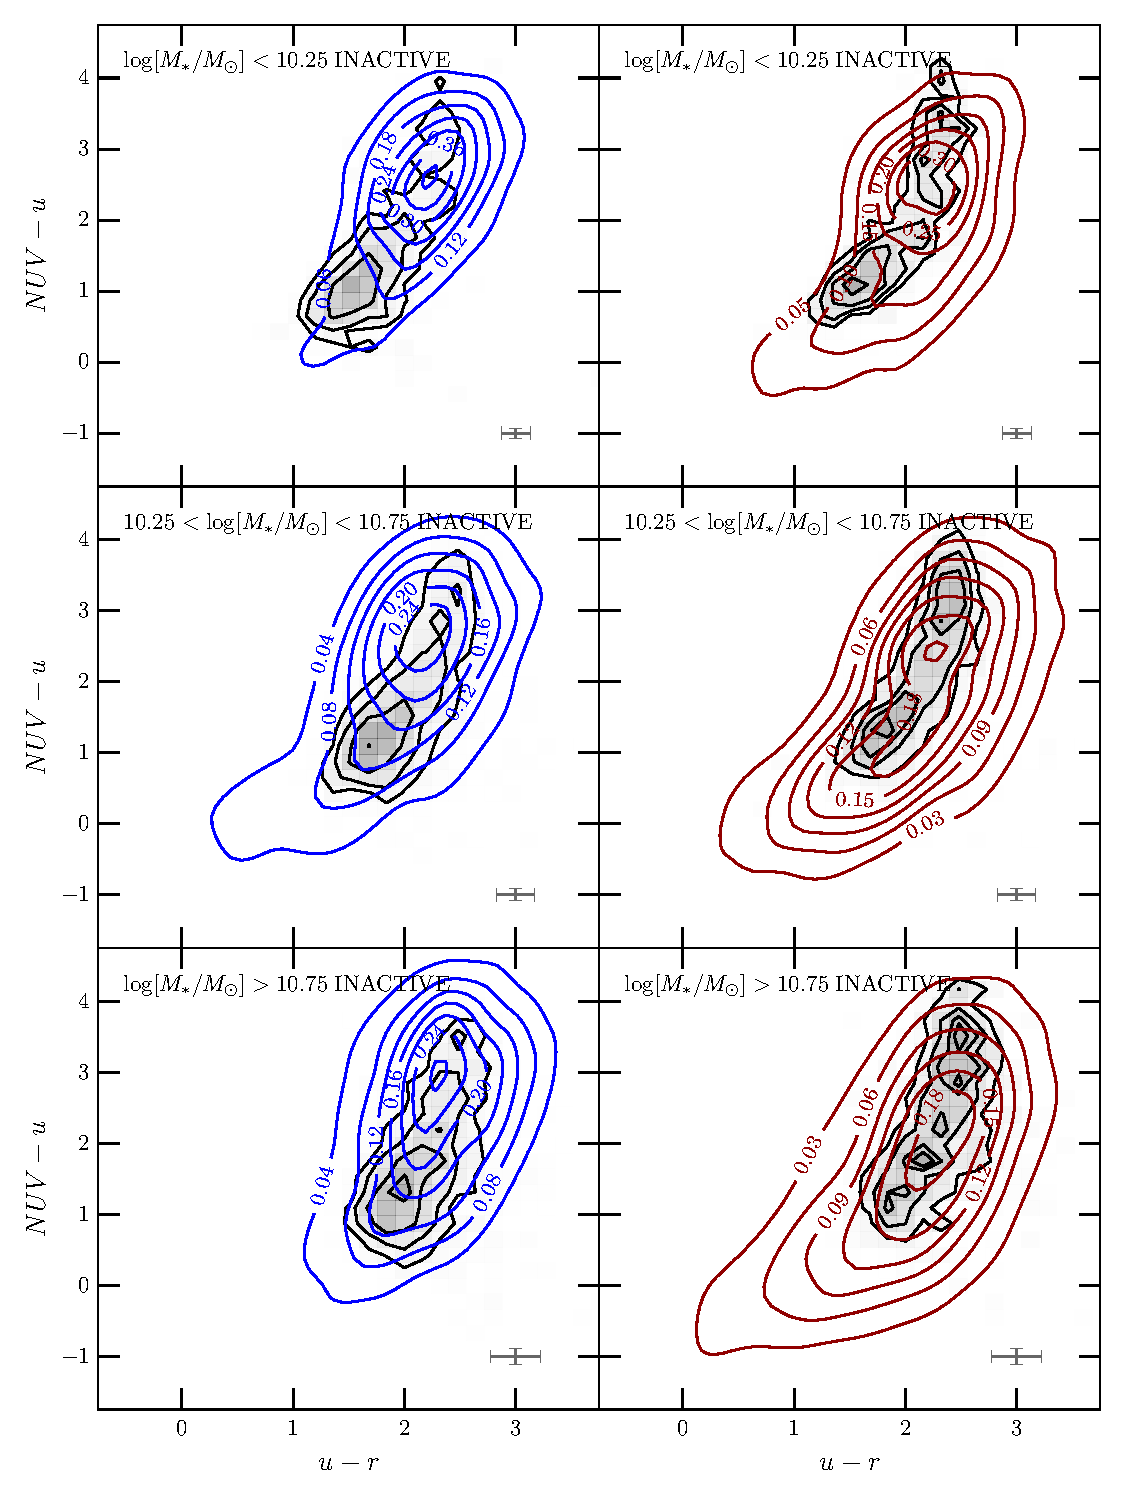
\includegraphics[width=0.7\textwidth]{starpy/inactive_colour_colour_hyper_generated_disc_inactive_distribution_kernel_samples_labelled.pdf}
\caption[Replica colour-colour distributions using a hierarchical method]{Optical-NUV colour-colour diagrams for the \textsc{inactive} {\minor sample of galaxies (defined in Section~\ref{sec:inactive} as a subset of the \textsc{gz2-galex} sample with all galaxies with line strengths indicative of potential AGN activity as defined by \citealt{kauffmann03b} and sources identified by \citealt{Oh15} as Type 1 AGN by the presence of broad emission lines removed)} shown by the black contours. The sample is split into low mass (top), medium mass (middle) and high mass (bottom) galaxies weighted by $p_d$ (left) and $p_s$ (right). Kernel smoothing has been applied to the overlaid replica datasets, which are created by sampling from the inferred 2 component Gaussian mixture model hierarchical parent distributions. Gaussian random noise is also added to the inferred colours, with a mean and standard deviation of the errors on the observed colours of the respective sample. Contours are shown for samples taken from the disc (blue) and smooth weighted (red) inferred hierarchical distributions. {\minor The underlying data contours bound $12\%$, $40\%$, $68\%$ and $86\%$ of the morphology weighted samples. The numbers show the contour levels for the overlaid replica data in each panel}.}
\label{replica}
\end{centering}
\end{figure}

\begin{figure}
\begin{centering}
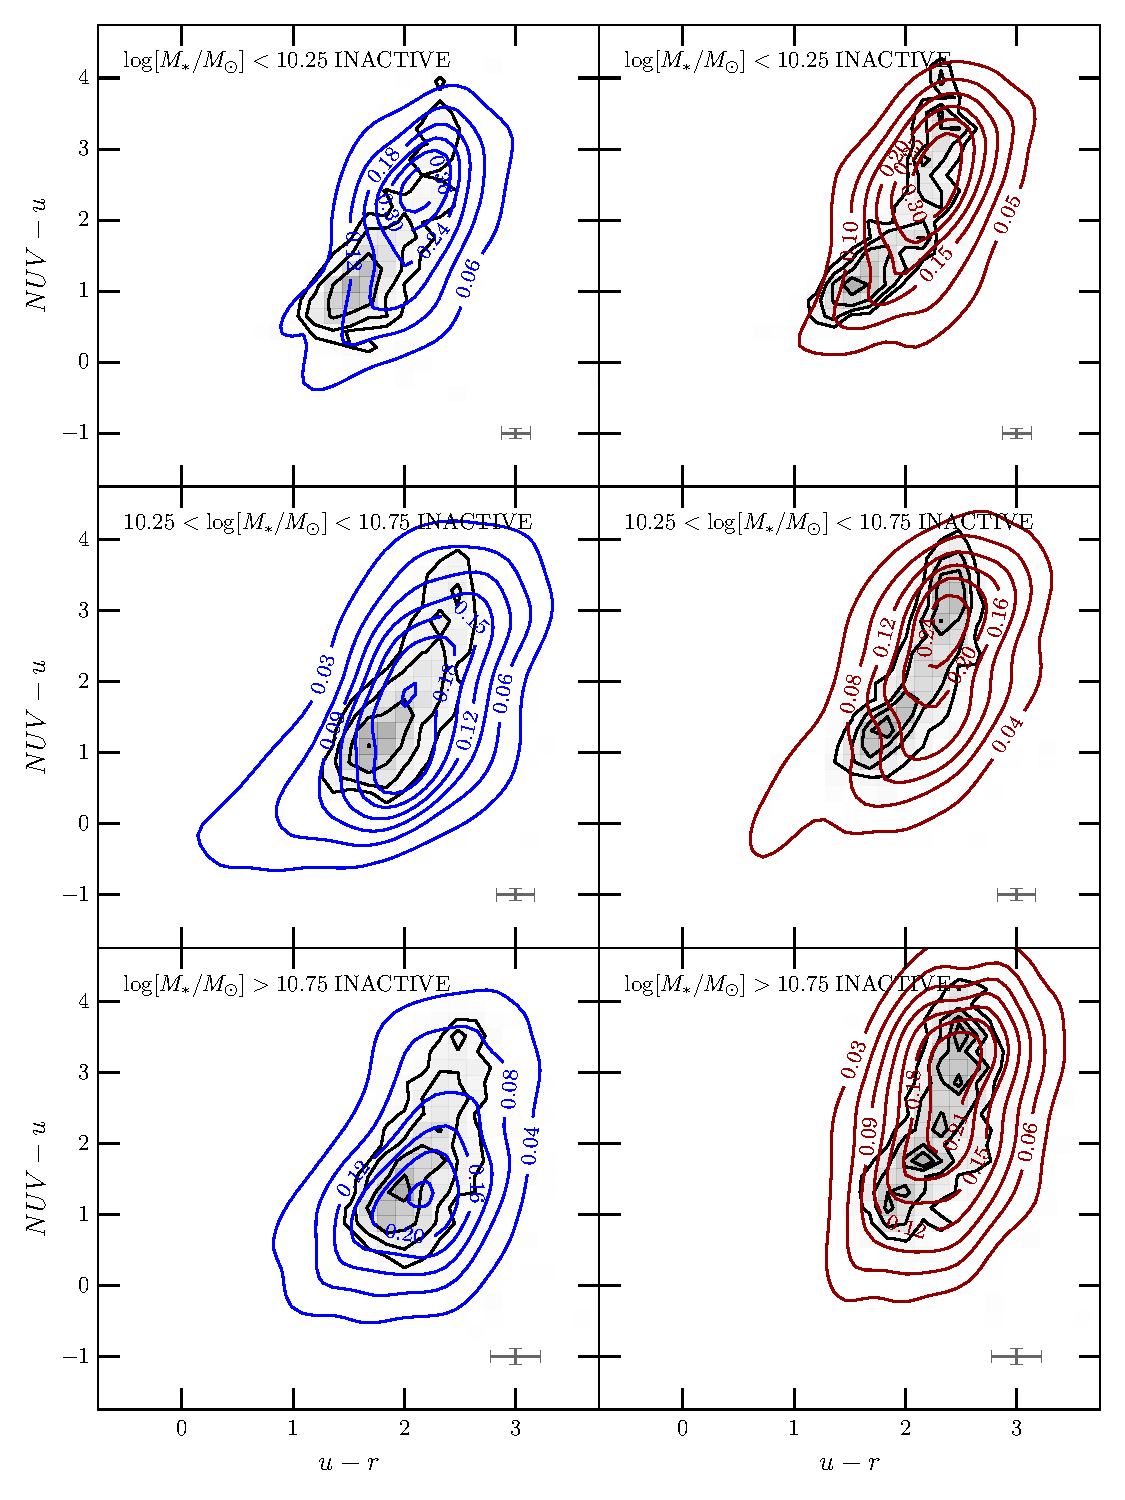
\includegraphics[width=0.7\textwidth]{starpy/inactive_colour_colour_popstarpy_generated_disc_distribution_contour_tq_ages_samples_no_log_weight_labelled.pdf}
\caption[Replica colour-colour distributions using the \textsc{popstarpy} method]{Optical-NUV colour-colour diagrams for the \textsc{inactive} {\minor sample of galaxies (defined in Section~\ref{sec:inactive} as a subset of the \textsc{gz2-galex} sample with all galaxies with line strengths indicative of potential AGN activity as defined by \citealt{kauffmann03b} and sources identified by \citealt{Oh15} as Type 1 AGN by the presence of broad emission lines removed)} shown by the black contours. The sample is split into low mass (top), medium mass (middle) and high mass (bottom) galaxies weighted by $p_d$ (left) and $p_s$ (right). Kernel smoothing has been applied to the overlaid replica datasets, which are created by sampling from the \textsc{popstarpy} population density distributions described in Section~\ref{popstarpy}. Gaussian random noise is also added to the inferred colours, with a mean and standard deviation of the errors on the observed colours of the respective sample. Contours are shown for samples taken from the disc (blue) and smooth weighted (red) inferred hierarchical distributions. {\minor The underlying data contours bound $12\%$, $40\%$, $68\%$ and $86\%$ of the morphology weighted samples. The numbers show the contour levels for the overlaid replica data in each panel}.}
\label{replicapop}
\end{centering}
\end{figure}

This approach is heavily dependent on what shape is assumed for the hyper-distribution; a decision which is not trivial. It is often common to assume the form of a multi-component Gaussian mixture model \citep{mackay03, lahav00}. For example a two component Gaussian mixture model in $[t_q, \tau]$ space is described by eight hyper-parameters for a single morphology, $\vec{\theta}' = [\mu_{t,1}, \sigma_{t,1}, \mu_{\tau,1}, \sigma_{\tau,1}, \mu_{t,2}, \sigma_{t,2}, \mu_{\tau,2}, \sigma_{\tau,2}]$. This approach assumes no covariance between hyper-parameters for simplicity. The equations outlined above, combined with MCMC methods can be used to infer these eight $\vec{\theta}'$ parameters from which the hierarchical population distribution can be determined. 

%I used this assumption of a two component Gaussian mixture model, to infer the population parameters for both the \textsc{agn-host} and \textsc{inactive} populations and the results are shown in Figure~\ref{method3}. These results were produced by drawing $N_s = 100$ random samples from each galaxy, $k$, in each mass bin. I plot the distributions for a given morphology by taking the median value of the posterior distribution for each of the 8 parameters describing the two component Gaussian mixture. I can see in Figure~\ref{method3} that this hierarchical method produces similar distributions for the \textsc{agn-host} and \textsc{inactive} samples. This finding is not expected given the differences between the two samples in colour-colour space seen in Figure~\ref{colcol}. 

%\begin{figure}
%\includegraphics[width=0.48\textwidth]{figc1a.pdf}
%\includegraphics[width=0.48\textwidth]{figc1b.pdf}
%\caption[8pt]{Hierarchical-posterior PDF of the quenching time ($t_q'$, top) and rate ($\tau'$, bottom) population parameters, normalised so that the areas under the curves are equal. \textsc{agn-host} (left) and \textsc{inactive} (right) galaxies are split into low (top), medium (middle) and high (bottom) mass, weighted for smooth (red dashed) and disc (blue solid) galaxies. A low (high) value of $t_q'$ corresponds to the early (recent) Universe. A small (large) value of $\tau'$ corresponds to a rapid (slow) quench.}
%\label{method3}
%\end{figure}

In order to test whether this assumption of a multi-component Gaussian mixture model is appropriate, I sampled the inferred hierarchical distributions to produce replica datasets in optical-NUV colour space. These are shown here in Figure~\ref{replica}  in comparison to the observed colour-colour distributions of the \textsc{inactive} sample (a subset of $\sim6,000$ galaxies from the \textsc{gz2-galex} sample, see Section~\ref{sec:agnfeedback}). For all masses and morphologies the replicated $u-r$ and $NUV-u$ colours do not accurately match the observed data. 


I also varied the value of $N_s$ and found that increasing the number of samples drawn did not improve this fit for the \textsc{inactive} population. Similarly increasing the number of components in the Gaussian mixture model did not immediately improve the accuracy of the fit along with other functional forms which require too many assumptions to be made about the shape of the parent distribution. I therefore concluded that assuming such a functional form of the population distribution was unsatisfactory. %An extensive exploration of a wide variety of functional forms is necessary to ensure the correct conclusions are drawn from the data. Such an investigation is beyond the scope of this paper. 

The \textsc{popstarpy} approach described in section \ref{popstarpy} was motivated by the investigation increasing the number of samples, $N_s$, drawn from the posterior of each galaxy, k, until the point where all the samples were drawn. Instead of attempting to infer parameters to describe this distribution, as above, I presented the combined distributions of all individual galaxies in a population (as described in Section \ref{popstarpy}).  The distributions produced by this visualisation method reveal the complexity that the parent distribution must describe which, as concluded earlier, cannot be effectively modelled.

I also tested whether the \textsc{popstarpy} method is reasonable by producing replica datasets in optical-NUV colour space, as before, by drawing $1000$ $[t_q, \tau]$ values from the population density distributions derived for the \textsc{inactive} sample (see Section~\ref{sec:agnfeedback}). These replica datasets are shown here in Figure~\ref{replicapop} in comparison to the observed colour-colour distributions of the \textsc{inactive} sample. Comparing these replica colours in Figure~\ref{replicapop}, with those produced by drawing from the inferred hierarchical distributions, shown in Figure~\ref{replica}, they can be seen to produce a more accurate match to the observed data for the majority of masses and morphologies. 

Considering these issues with assuming a functional form for the hierarchical parent distribution, an expansion on this approach would be to perform `heat map optimization', similar to image reconstruction, to determine the parent distribution for a given population. The population parameter space would be divided into an $M \times M$ grid of pixels and the value of each pixel would be a model parameter to be inferred by hierarchical Bayesian methods. Each pixel would need a prior (e.g. a basic entropic prior) and the heat map would sum to unity. In order for this pixel map to accurately characterise the detail expected in the parent populations, this pixel grid would need to be sufficiently large, with at least a $50\rm{x}50$ grid of pixels (i.e. upwards of $2500$ model parameters, $\theta'$, to be inferred). This is a significant expansion upon the work presented here and is something I wish to investigate in future work (see Section~\ref{sec:future}).

For the results presented in Chapters~\ref{chap:morph} \& \ref{chap:agn}, I therefore use the \textsc{popstarpy} method to visualise the population distribution, rather than quoting inferred values to describe it.


